\documentclass{standalone}
\usepackage{tikz}
\usepackage{ctex,siunitx}
\setCJKmainfont{Noto Serif CJK SC}
\usepackage{tkz-euclide}
\usepackage{amsmath}
\usetikzlibrary{patterns, calc,3d}
\usetikzlibrary {decorations.pathmorphing,decorations.pathreplacing,decorations.shapes}
\begin{document}
\small
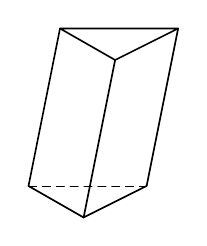
\begin{tikzpicture}[>=latex,scale=1.0]
  \tkzDefPoints{0/0/A,1.5/0/B,0.7/-0.4/C,0.4/2.0/A'}
  \tkzDefPointsBy[translation=from A to A'](B,C){B',C'}
  \tkzDrawPolygon[semithick](A',B',C')
  \tkzDrawSegments[densely dashed](A,B)
  \tkzDrawSegments[semithick](A,A' B,B' C,C' A,C B,C)
\end{tikzpicture}
\end{document}